% Appendix Template

\chapter{Tutorial de como utilizar el software \textit{Petrinator}} % Main appendix title

\label{AppendixA} % Change X to a consecutive letter; for referencing this appendix elsewhere, use \ref{AppendixX}
En este apéndice, se detalla el procedimiento en el cual se crean y cargan redes de Petri para trabajar con ellas con dicho software.
Luego se explica el procedimiento que se debe seguir para extraer los datos necesarios para el análisis del algortimo.


\section{Ejecución del software}

A continuación explican los pasos que se deben seguir para poder iniciar el agente \textit{Petrinator} en el dispositivo. 

\begin{itemize}   
    \item  \textbf{Ingreso al programa:}
    desde la terminal de linux \footnote{La ejecución del software tambien puede realizarse en Windows. Para ambos casos es necesario instalar los paquetes correspondientes de java.} se ejecuta el comando: 
    \begin{lstlisting}[language=SHELXL]
    		$ java -jar Petrinator.jar
    \end{lstlisting}
    
    \begin{figure} [H]
        \centering
        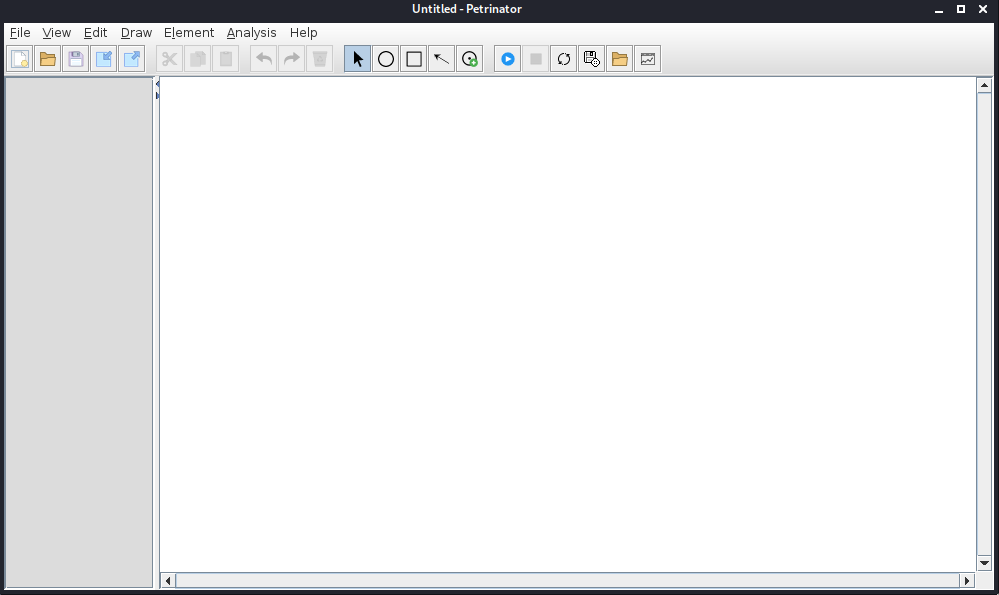
\includegraphics[width=\textwidth]{Figures/petrinator/petrinator-init.png}
        \caption{Software Petrinator .}
        \label{fig:pet-init}
    \end{figure}
   
    \item \textbf{Cargar la red de Petri:} una vez ejecutado exitosamente, se deberá importar o crear la red a analizar. Como se muestra en la figura \ref{fig:file-open}.
    
	\begin{figure} [H]
        \centering
        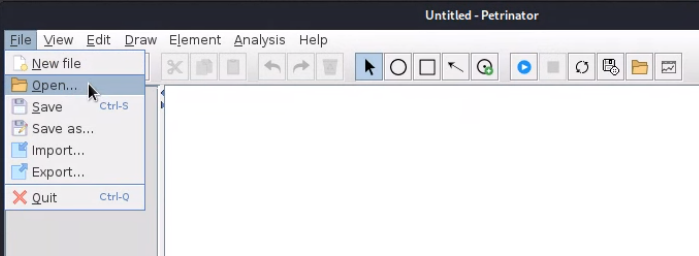
\includegraphics[scale=0.72]{Figures/petrinator/open2.png}
        \caption{Abrir un archivo .}
        \label{fig:pet-open}
    \end{figure} 
    
    \noindent Seleccionar el archivo de extensión \textit{.pflow} a cargar
    \begin{figure} [H]
        \centering
        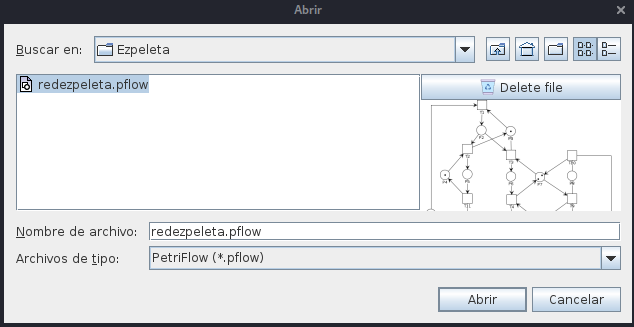
\includegraphics[scale=0.7]{Figures/petrinator/open-example.png}
        \caption{Ventana de selección de archivo .pflow .}
        \label{fig:file-open}
    \end{figure}
    
    \begin{figure} [H]
        \centering
        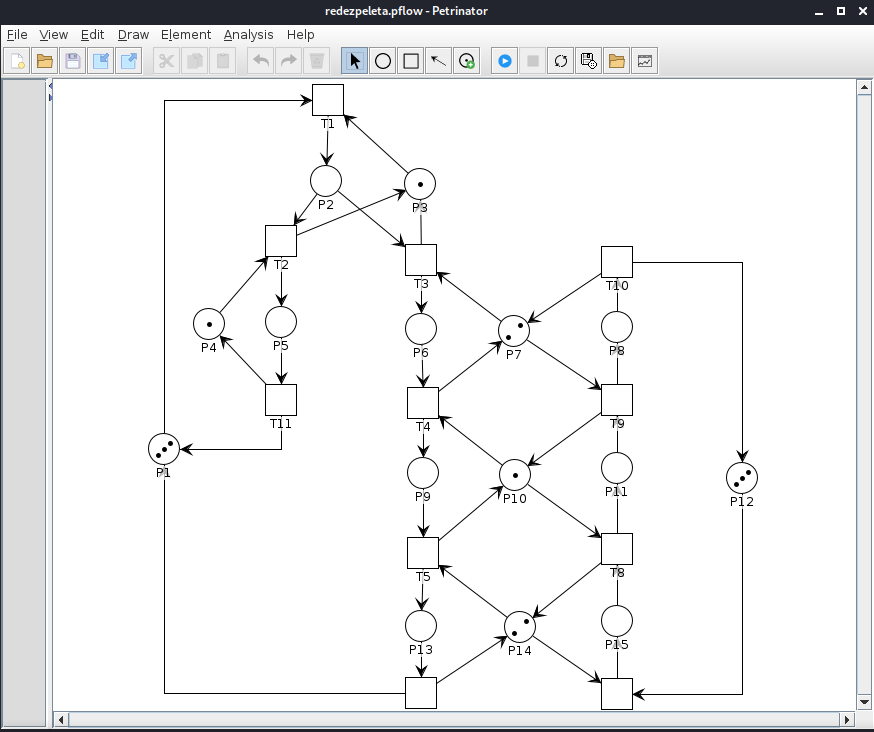
\includegraphics[scale=0.45]{Figures/petrinator/open-example2.png}
        \caption{Red cargada .}
        \label{fig:red-open}
    \end{figure}
    
	
    \item \textbf{Extraer archivos para el análisis:} Como se puede observar en la figura \ref{fig:open-analysis}, en la barra de menú se encuentra la opción de \textit{Analysis} desde donde se pueden realizar los diferentes tipos de análisis en las redes de Petri. A partir de estos, se extraen 4 diferentes archivos.
    
    \begin{figure} [H]
        \centering
        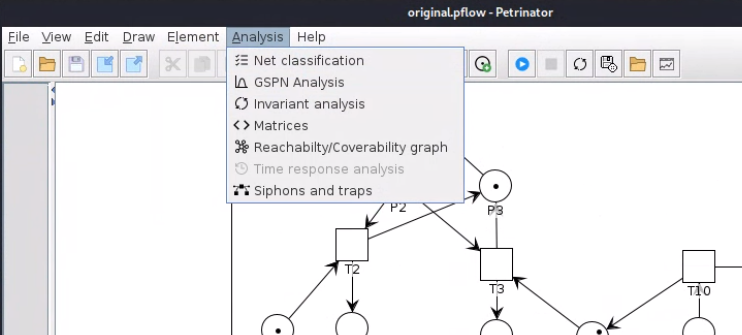
\includegraphics[scale=0.7]{Figures/petrinator/analisis.png}
        \caption{Submenú de análisis.}
        \label{fig:open-analysis}
    \end{figure}
    
    \begin{itemize}
        \item \textbf{Clasificación de la red}: como se observa en la figura \ref{fig:open-analysis} se encuentra en el submenú la opción \textit{Net classification} que nos permite realizar este análisis.
        Una vez seleccionada la opción, se abre una nueva ventana como muestra la figura \ref{fig:clasificacion-red} en dónde se debe pulsar en \textit{Classify} para que el software haga dicho análisis. Para la funcionalidad de nuestro algoritmo no es necesario exportar este archivo, sin embargo es de imprescindible verificar la presencia de Deadlock. En caso de haber bloqueo es necesaria la extracción de los siguientes archivos para la ejecución del algoritmo; en caso contrario no sería una red de interés.
        
        \begin{figure} [H]
            \centering
            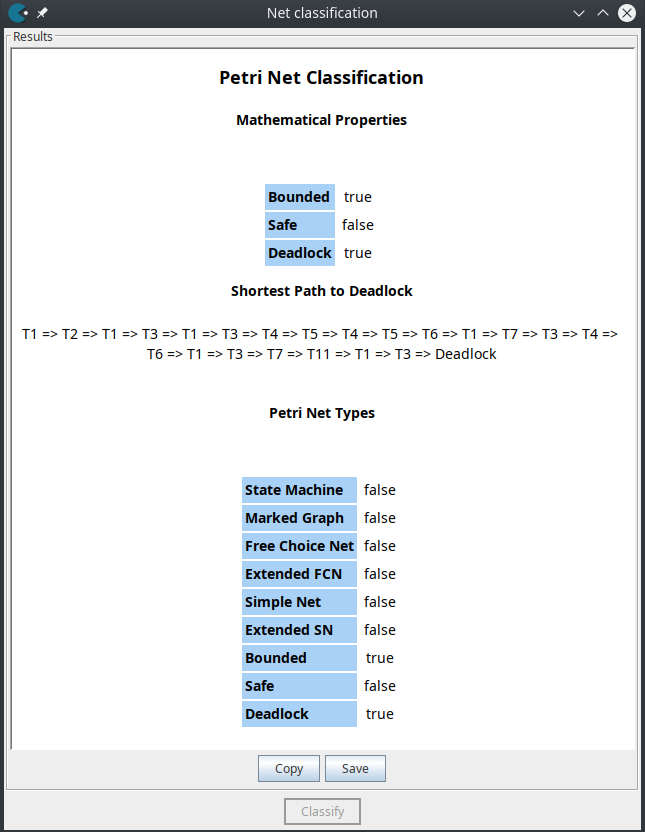
\includegraphics[scale=0.5]{Figures/petrinator/net_clasification.png}
            \caption{Clasificación y propiedades de la red .}
            \label{fig:clasificacion-red}
        \end{figure}
        
        \item \textbf{Análisis de Invariantes}: como se observa en la figura \ref{fig:open-analysis} se encuentra en el submenú la opción \textit{Invariant analysis} que nos permite realizar este análisis.
        Una vez seleccionada la opción, se abre una nueva ventana como muestra la figura \ref{fig:ext-inv} en dónde se debe pulsar en \textit{Analyse} para que el software haga dicho análisis y luego en \textit{Save}.
        
        \begin{figure} [H]
            \centering
            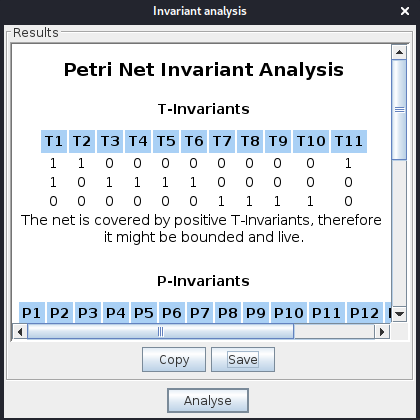
\includegraphics[scale=0.7]{Figures/petrinator/invariantes.png}
            \caption{Exportar invariantes.}
            \label{fig:ext-inv}
        \end{figure}
        
        \item \textbf{Matrices:} como se observa en la figura \ref{fig:open-analysis} se encuentra en el submenú la opción \textit{Matrices} que nos permite calcular las matrices asociadas a la red.
        Una vez seleccionada la opción, se abre una nueva ventana como muestra la figura \ref{fig:ext-mat} en dónde se debe pulsar en \textit{Calculate} para que el software haga los cálculos y luego en \textit{Save}.
        \begin{figure} [H]
            \centering
            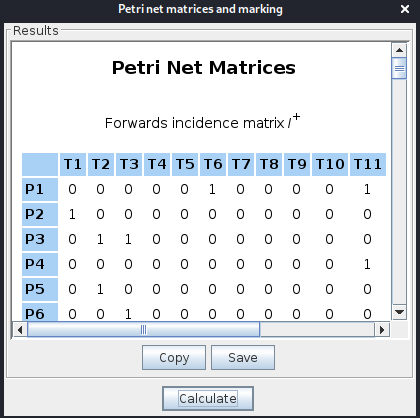
\includegraphics[scale=0.7]{Figures/petrinator/matrices.png}
            \caption{Exportar matrices.}
            \label{fig:ext-mat}
        \end{figure}
        
        \item \textbf{Grafo de Alcanzabilidad}: como se observa en la figura \ref{fig:open-analysis} se encuentra en el submenú la opción \textit{Reachability/Coverability graph} que nos permite generar el grafo con todos los estados alcanzables de la red.
        Una vez seleccionada la opción, se abre una nueva ventana como muestra la figura \ref{fig:ext-grafo} en dónde se debe pulsar en \textit{Generate states} para que el software genere dicho análisis y luego en \textit{Save}.
        \begin{figure} [H]
            \centering
            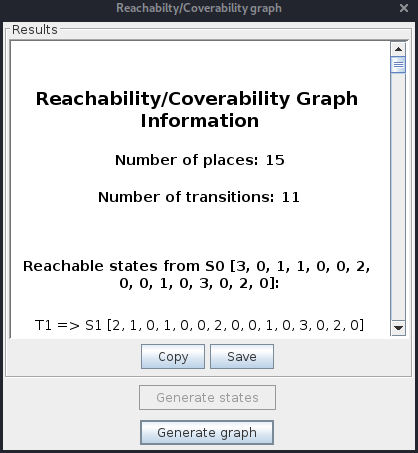
\includegraphics[scale=0.7]{Figures/petrinator/grafo.png}
            \caption{Exportar grafo de alcanzabilidad.}
            \label{fig:ext-grafo}
        \end{figure}
        
        \item \textbf{Sifones y Trampas}: como se observa en la figura \ref{fig:open-analysis} se encuentra en el submenú la opción \textit{Siphons and traps} que nos permite calcular todos los sifones y trampas presentes en la red.
        Una vez seleccionada la opción, se abre una nueva ventana como muestra la figura \ref{fig:ext-tys} en dónde se debe pulsar en \textit{Analyse} para que el software realice el cálculo y luego en \textit{Save}.
        \begin{figure} [H]
            \centering
            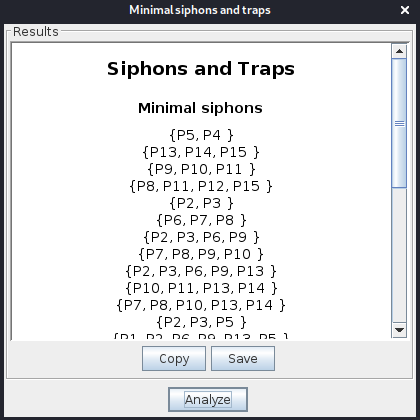
\includegraphics[scale=0.7]{Figures/petrinator/sifones.png}
            \caption{Exportar sifones y trampas.}
            \label{fig:ext-tys}
        \end{figure}
        
    \end{itemize}
    
  
\end{itemize}